\section{Conception et implémentation}\label{sec:conception_implementation}
    \subsection{Conception et implémentation des chases}
        \subsubsection{Analyse de l'existant dans Graal}
        \begin{figure}[H]
        \centering
        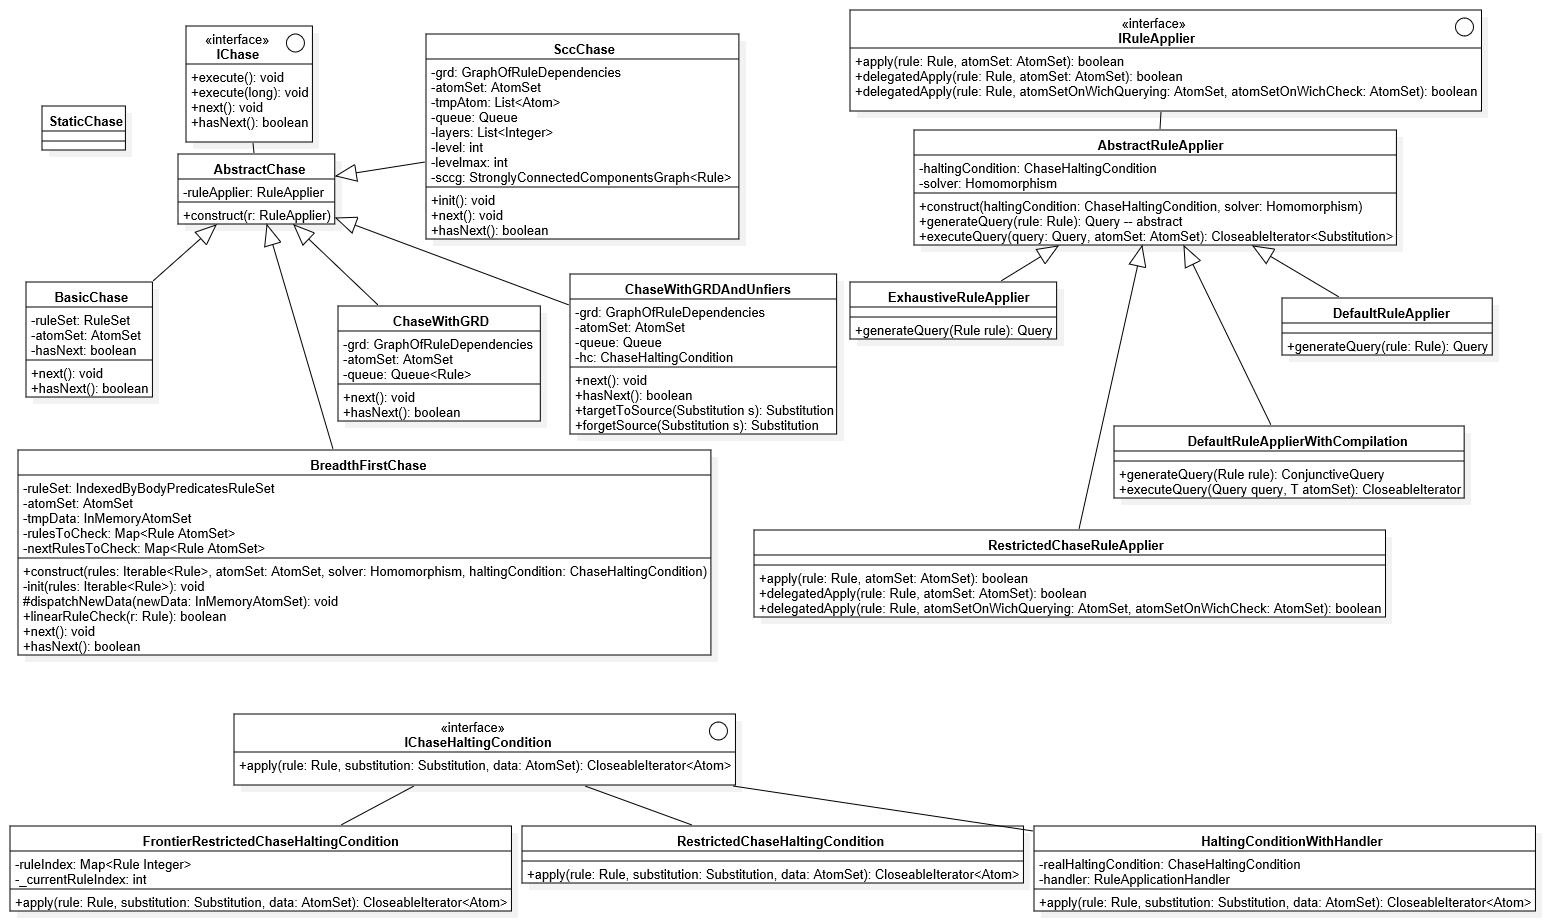
\includegraphics[width=\textwidth]{pictures/DiagrammeClasse.png}
        \caption{Diagramme de classes GRAAL}
        \label{fig:dclasse}
        \end{figure}
        
        Dans cette partie nous analysons ce qui était déjà présent sur GRAAL pour les \textit{chases}.
        
        Le package graal-forward-chaining est compris par 3 packages :
        \begin{itemize}
            \item \textit{Chase} : Il contient les implémentations des différentes \textit{chases} ( BreadthFirst, GRD, etc )
            \item \textit{HaltingCondition} : Une halting condition sert à tester si un trigger (R,h) est "actif" et s'il l'est la règle est appliquée par rapport à h.
            \item \textit{RuleApplier} : Un rule applier sert à calculer tous les homomorphismes du Body d'une règle dans F et ensuite il utilise les homomorphismes trouvés pour appliquer la règle en utilisant une \textit{HaltingCondition}.
        \end{itemize}
        
        \paragraph{Package Chase}\ \\
        Le package \textit{Chase} est compris d'une interface \textit{IChase} étant implementé par tous les \textit{chases} dans GRAAL. D'une classe abstraite AbstractChase qui implemente des versions génériques pour les méthodes de \textit{chases}. Enfin on a les différentes classes implementant different type de \textit{chases}.\\
        Le \textit{BasicChase} est une implémentation basique du \textit{chases} en largeur sans aucune optimisation. \\
        Le \textit{BreadthFirstChase} est une implémentation optimisée du \textit{chase} en largeur. Une première optimisation est l'utilisation de \textit{nouvFaits} à la fin de chaque étape pour déterminer quelles règles seront déclenchées à l'étape prochaine. On détermine aussi parmi ces règles lesquelles sont linéaires (avec un seul atome dans le body) pour stocker les atomes à utiliser pour le calcul des homomorphismes de façon à ce que ce dernier prenne en entrée une petite collection d'atomes plutôt que la base la base de faits entière. \\
        Le \textit{ChaseWithGRD} est un \textit{chase} qui utilise le graphe de dépendance des règles.\\
        Le \textit{SccChase} est un \textit{Chase} qui sature chaque composante fortement connexe du graphe de dépendance des règles individuellement. on l'utilise par la classe statique \textit{StaticChase}.\\
        Enfin le \textit{ChaseWithGRDAndUnfiers} est un \textit{chase} utilisant le graphe de dépendance des règles et des unificateurs.
        
        %\begin{itemize}
            %\item IChase : Interface qui doit être implémenté par tous les chases dans GRAAL.
            %\item AbstractChase : Classe abstraite qui implémente des versions génériques pour les méthodes des chases.
            %\item BasicChase : Implémentation basique du chase en largeur sans aucune optimisation.
            %\item BreadthFirstChase : Implémentation optimisée du chase en largeur. Une première optimisation est l'utilisation de nouvFaits à la fin de chaque étape pour déterminer quelles règles seront déclenchées à l'étape prochaine. On détermine aussi parmi ces règles lesquelles sont linéaires (avec un seul atome dans le body) pour stocker les atomes à utiliser pour le calcul des homomorphismes de façon à ce que ce dernier prenne en entrée une petite collection d'atomes plutôt que la base la base de faits entière.
            %\item ChaseWithGRD : Chase qui utilise le graphe de dépendance des règles.
            %\item SccChase : Chase qui sature chaque composante fortement connexe du graphe de dépendance des règles individuellement.
            %\item StaticChase : Classe statique qui permet d'utiliser le SccChase.
            %\item ChaseWithGRDAndUnfiers : Chase utilisant le graphe de dépendance des règles et des unificateurs.
        %\end{itemize}
        
        \paragraph{Package Halting Condition}\ \\
        Le package Halting Condition permet normalement de définir les différentes conditions d'arrêt pour la saturation des \textit{chases}. Mais ici un Halting condition teste plutôt si un trigger est actif avant de l'appliqué le cas échéant.\\ 
        Il est composé de l'interface IChaseHaltingCondition qui est implémenté par toutes les halting conditions. On ainsi deux classes:\\
        La FrontierRestrictedChaseHaltingCondition est utilisée par le semi-oblivious chase. \\
        La RestrictedChaseHaltingCondition est utilisée par le restricted chase.
        %\begin{itemize}
            %\item IChaseHaltingCondition : Interface à implémenter pour toutes les halting conditions. 
            %\item FrontierRestrictedChaseHaltingCondition : HaltingCondition utilisée par le semi-oblivious chase.
            %\item RestrictedChaseHaltingCondition : HaltingCondition utilisée par le restricted chase.
        %\end{itemize}

        \paragraph{Package RuleApplier}\ \\
        Le package RuleApplier est le package qui définit comment se s'applique les règles lors d'un \textit{chase}. Il est composé de l'interface IRuleApplier qui est implementée par tous les rules appliers. Nous avons ici 4 classes de rule applier:\\
        Le DefaultRuleApplier calcule tous les homomorphismes puis ne garde que la frontière de chacun.\\
        L'ExhaustiveRuleApplier calcule tous les homomorphismes et les garde sans aucune modification.\\
        Le RestrictedChaseRuleApplier est spécifiquement optimisé pour le restricted chase.\\
        Le DefaultRuleApplierWithCompilation est un Rule Applier qui utilise des règles avec compilation.
        
        %\begin{itemize}
            %\item IRuleApplier : Interface à implémenter pour tous les rules appliers. 
            %\item DefaultRuleApplier : Il calcule tous les homomorphismes puis ne garde que la frontière de chacun.  
            %\item ExhaustiveRuleApplier : Il calcule tous les homomorphismes et les garde sans aucune modification.
            %\item RestrictedChaseRuleApplier : Rule Applier spécifiquement optimisé pour le restricted chase. 
            %\item DefaultRuleApplierWithCompilation : Rule Applier qui utilise des règles avec compilation.
        %\end{itemize}
        
        \begin{figure}[H]
        \centering
        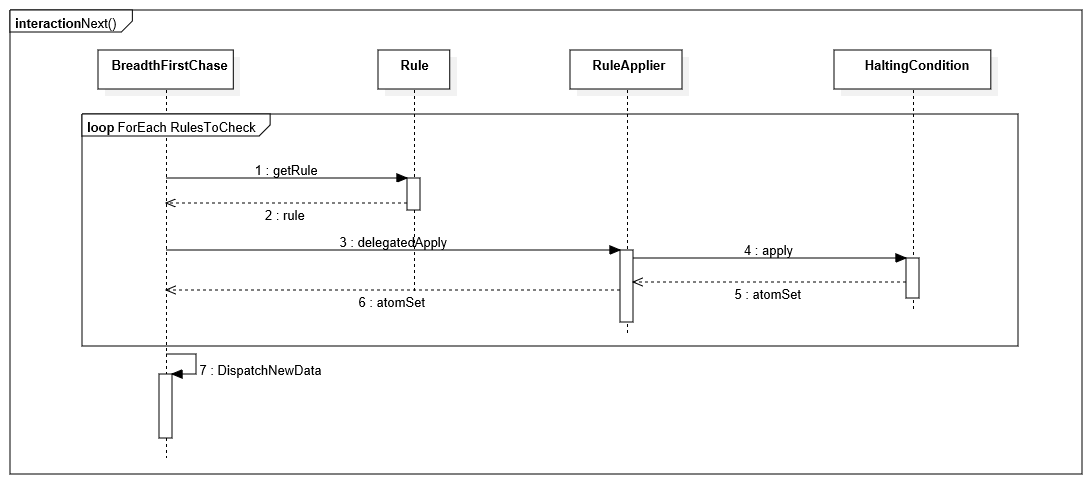
\includegraphics[width=\textwidth]{pictures/DiagrammeSequence.png}
        \caption{Diagramme de sequence next()}
        \label{fig:dsequence}
        \end{figure}
        
        Pour que le diagramme de sequence et donc le fonctionnement des chases soit plus comprehensible il nous semblait important de revenir sur la fonction \textit{next()} et sur son fonctionnement.
        
        \paragraph{Fonction \textit{next()}}\ \\
        La fonction next() fait une étape de largeur de l'algorithme chase en parallèle. Cette fonction utilise deux hashmaps du type Map<Rule, AtomSet> pour stocker les règles qui devront être appliquées à l'étape suivante et les atomes qui seront utilisés pour le calcul des homomorphismes, ces deux hashmaps s'appellent rulesToCheck et nextRulesToCheck. Avant le premier appel à la méthode on initialise nextRulesToCheck avec toutes les règles de la base de règles de la façon suivante : $nextRulesToCheck({R}) = <{R},\mathcal{F}> $. À chaque appel de la méthode next on suit les étapes suivantes : 
        \\
        
        \begin{itemize}
        \item On copie $nextRulesToCheck$ dans $rulesToCheck$, et on réinitialise $nextRulesToCheck$.
        \item Pour chaque règle $R_i$ dans $rulesToCheck$ on appelle la fonction $delegatedApply$ dans RuleApplier qui va calculer tous les homomorphismes du corps de la règle vers la base de faits de l'étape précédente, puis, pour chacun de ces homomorphismes on appelle la fonction $apply$ dans HaltingCondition et on génère les atomes s'ils ne sont pas redondants par rapport au critère choisi, c'est-à-dire, on applique l'homomorphisme à la tête de la règle.
        \item Les atomes génerés par HaltingCondition sont renvoyés au BreadthFirstChase à travers RuleApplier. Ces atomes sont stockés par BreadthFirstChase dans nouvFaits puis on continue avec la règle suivante.
        \item Quand on a traité toutes les règles on appelle $dispatchNewData$ qui va prendre tous les nouveaux atomes générés, et pour chacun de ces atomes cette fonction teste sur chacune des règles de $\mathcal{BR}$ si cet atome $\alpha$ apparaît dans le corps de la règle. 
        \item S'il n'appartient pas au corps de la règle on continue avec la règle suivante, mais s'il appartient on a deux cas; soit la règle n'est pas linéaire alors on l'ajoute dans $nextRulesToCheck(R_i,\mathcal{BF})$, soit elle est linéaire et n'a pas déjà été ajoutée dans $nextRulesToCheck$ dans ce cas on l'ajoute dans $nextRulesToCheck(R_i, \alpha)$. Sinon on ajoute l'atome $\alpha$ dans la liste associé à la règle dans $nextRulesToCheck(R_i)$. 
        \end{itemize}
        
        \paragraph{Critique}
        Face à cette organisation et dans l'idée de proposer notre propre itération d'une implémentation des chases  nous avons donc était amené à nous demandé qu'elles étaient les choses pouvant être améliorées.\\
        Tout d'abord le nom du package HaltingCondition n'est pas le plus clair, une halting condition devrait normalement être une condition d'arrêt pour la saturation d'un chase, mais ici, elles testent si un trigger est actif et ensuite l'appliquent.\\
        Ensuite nous avons remarqué que l'implémentation génériques des chases n'utilisé pas les notions d'extensions locale et d'extensions globale, GRAAL fait toujours l'union ce qui pourrait être amélioré.\\
        Nous avons aussi remarqué qu'il existe des classes qui ne sont pas utiles ou pas encore finies. StaticChase ou HaltingConditionWithHandler en sont des exemples.\\
        Enfin nous nous sommes rendus compte que dans l'implémentation actuelle de Graal, les homomorphismes sont recalculés intégralement à chaque étape du chase, ce qui ralentit considérablement le calcul de la base de faits saturée.
        %\begin{itemize}
            %\item Nous ne trouvons pas que le package HaltingCondition est bien nommé, une halting condition devrait normalement être une condition d'arrêt pour la saturation d'un chase, mais ici, elles testent si un trigger est actif et ensuite l'appliquent.
            %\item Pour avoir des implémentions vraiment génériques des chases il faudrait rajouter les notions d'extension locale et d'extension globale, Graal fait toujours l'union.
            %\item Il existe des classes qui ne sont pas utiles ou pas encore finies. StaticChase ou HaltingConditionWithHandler en sont des exemples. 
            %\item Dans l'implémentation actuelle de Graal, les homomorphismes sont recalculés intégralement à chaque étape du chase, ce qui ralentit considérablement le calcul de la base de faits saturée.
        %\end{itemize}
        
        %\subsubsection{Conception}
     %\subsection{Conception et implémentation des simplificateurs de bases de règles}
     
     
    \subsubsection{Analyse du nouveau travail dans Graal}
        \begin{figure}[H]
        \centering
        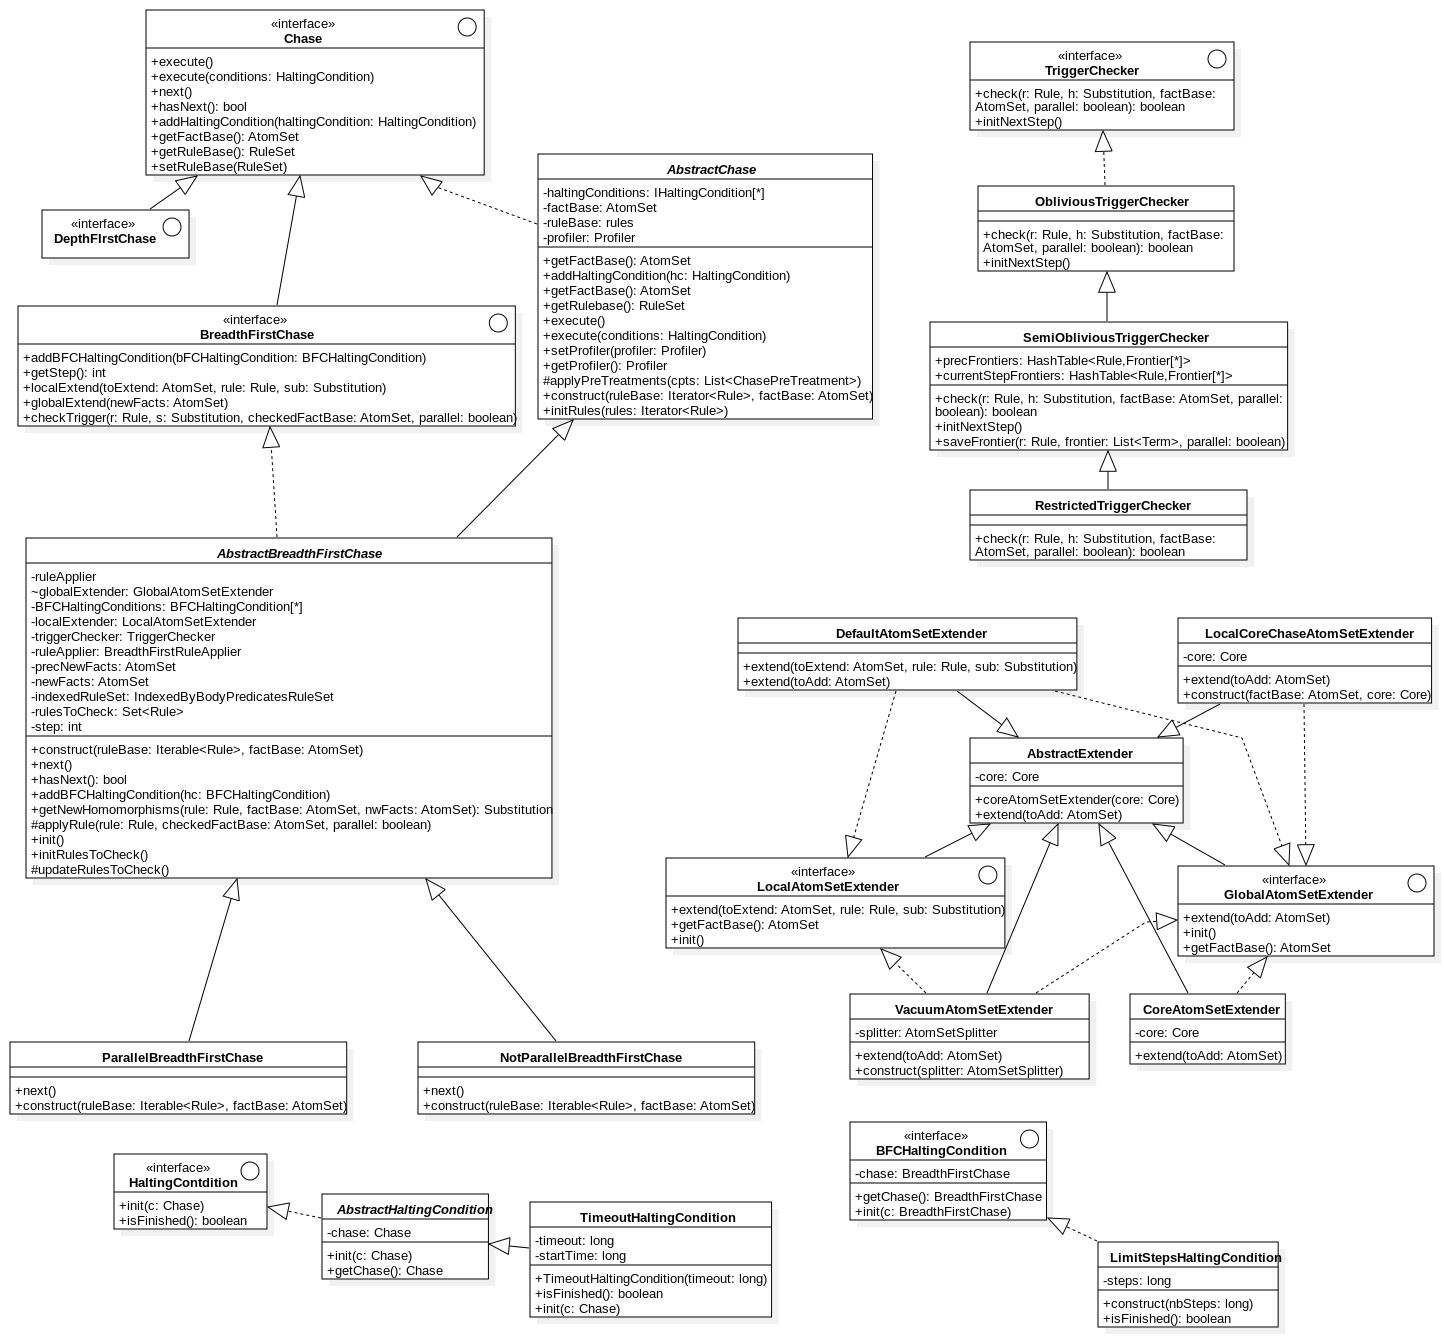
\includegraphics[width=\textwidth]{pictures/NouveauDiagrammeClasse.png}
        \caption{Nouveau Diagramme de classes GRAAL // needs updating}
        \label{fig:dclasse}
        \end{figure}
        
    Dans cette partie nous développerons le travail que nous avons fait sur l'implémentation des \textit{chases} que nous proposons. L'organisation des classes, les fonctions utilisées et de manière générale les problèmes que nous avons rencontré et au final comment cette nouvelle version est sensée fonctionner.
    
    \paragraph{Package Chase}\ \\
    Pour l'implémentation des \textit{chases} nous avons mis en place une interface Chase reprenant les fonctions \textit{execute()} et \textit{execute(HaltingCondition)} servant à exécuter l'algorithme \textit{chase} en ajoutant un condition d'arrêt.
    Cette interface est héritée par la classe abstraite \textit{AbstractChase} qui implémente les versions générique des \textit{chases}. On a aussi l'interface \textit{BreadthFirstChase} (resp. \textit{BreadthFirstChase}) qui représente l'interface qui doit être implémentée par les \textit{chases} en largeur (resp.profondeur).
    Enfin on a la classe \textit{classicBreadthFirstChase} fonctionnant pour les exécutions en largeur et la classe \textit{ParralelBreadthFirstChase} fonctionnant pour les exécutions en parallèle. On a fait la différence entre les deux parce que la version en parallèle n’est pas affecté par l’ordre d’application de règles alors qu'une version en largeur est sensible à l’ordre d’application de règles.
        %\begin{itemize}
            %\item Chase : Interface qui doit être implémentée par tous les chases dans GRAAL.
            %\item AbstractChase : Classe abstraite qui implémente des versions génériques pour les méthodes des chases.
            %\item DepthFirstChase : Interface qui doit être implémentée par tous les chases en profondeur.
            %\item BreadthFirstChase : Interface qui doit être implémentée par tous les chases en largeur.
            %\item AbstractBreadthFirstChase : Classe abstraite qui implémente des versions génériques pour les méthodes des chases en largeur.
            %\item ParallelBreadthFirstChase : Classe qui implémente les chases en parallèle.
            %\item NotParallelBreadthFirstChase : Classe qui implémente les chases en largeur.
        %\end{itemize}
        
    \paragraph{Package Trigger Checker}\ \\
    Pour le test d'applicabilité des règles nous avons mis en place une interface \textit{TriggerChecker} reprenant la fonction \textit{check} qui nous répond par vrai si une règle donnée est applicable pour un homomorphisme et la base de faits données et faux sinon. Et nous avons différentes classes pour les différents implémentations pour le test d'applicabilité. La classe qui vérifie l'applicabilité de l'Oblivious chase par la méthode check et donc va retourner toujours vrai. Voir l'algorithme \ref{algo:est_applicable_oblivious}. La classe qui étend l'ObliviousTriggerChecker en vérifiant l'applicabilité du SemiOblivious chase par la méthode check. Voir l'algorithme \ref{algo:est_applicable_semi_oblivious}. Et finallement la classe qui étend le SemiObliviousTriggerChecker en  vérifiant l'applicabilité du Restricted chase par la méthode check. Voir l'algorithme \ref{algo:est_applicable_restricted}.
        \\
        %\begin{itemize}
            %\item TriggerChecker : Interface qui doit être implémenté par tous les TriggerChecker dans GRAAL.
            %\item ObliviousTriggerChecker : Classe qui vérifie l'applicabilité de l'Oblivious chase par la méthode check. Voir l'algorithme \ref{algo:est_applicable_oblivious}. % retourne toujours vrai
            %\item SemiObliviousTriggerChecker : Classe qui étend l'ObliviousTriggerChecker en  vérifiant l'applicabilité du SemiOblivious chase par la méthode check. Voir l'algorithme \ref{algo:est_applicable_semi_oblivious}.
            %\item RestrictedTriggerChecker : Classe qui étend le SemiObliviousTriggerChecker en  vérifiant l'applicabilité du Restricted chase par la méthode check. Voir l'algorithme \ref{algo:est_applicable_restricted}.
        %\end{itemize}
        
    \paragraph{Package Halting Condition}\ \\
    Pour éviter les cas où l'exécution d'un \textit{chase} ne termine pas, nous avons dû ajouter un condition d'arrêt. On a mis en place une interface \textit{HaltingCondition} (resp. \textit{BFCHaltingCondition}) reprenant la fonction \textit{isFinished} qui nous dit si l'exécution des \textit{chases} (resp. en largeur) est terminée ou non. \textit{HaltingCondition} (resp. \textit{BFCHaltingCondition}) est héritée par la classe abstraite \textit{AbstractHaltingCondition} (resp. \textit{AbstractBFCHaltingCondition}) qui implémente les conditions d'arrêt pour les différents \textit{chases} (resp. \textit{chases} en largeur). On a deux conditions d'arrêt la première consiste à tester si l'exécution a dépassé un certain nombre d'étapes c'est pourquoi on a la classe \textit{LimitStepsHaltingCondition} et la seconde avec la classe \textit{TimeoutHaltingCondition} consiste à tester si l'exécution a dépassé un certain temps donné.
        %\begin{itemize}
            %\item HaltingCondition : Interface qui doit être implémentée pour définir les différentes conditions d'arrêt dans GRAAL.
            %\item BFCHaltingCondition : Interface qui doit être implémenté pour définir les conditions d'arrêt des chases en largeur dans GRAAL.
            %\item LimitStepsHaltingCondition : Classe qui implémente la condition d'arrêt par nombres d'étapes.
            %\item AbstractHaltingCondition : Classe abstraite qui implémente les conditions d'arrêt pour les différents chases.
            %\item AbstractBFCHaltingCondition : Classe abstraite qui implémente les conditions d'arrêt pour les différents chases en largeur.
            %\item TimeoutHaltingCondition : Classe qui implémente la condition d'arrêt par rapport au temps d'exécution.
        %\end{itemize}
        
        
    \paragraph{Package Rule Applier}\ \\
    Après le test d'applicabilité, si une règle est applicable il faut l'appliquer. Pour l'application des règles on a mis en place une interface \textit{BreadthFirstRuleApplier} qui implemente une classe abstraite \textit{AbstractBreadthFirstRuleApplier} qui sert pour l'implementation des \textit{chases} en largeur, ainsi que deux classes \textit{DefaultBreadthFirstRuleApplier} et \textit{RestrictedBreadthFirstRuleApplier} qui reprenent la fonction \textit{applyRule}. Cette dernière applique la règle déjà validée par le \textit{Trigger Checker}.     
        %\begin{itemize}
            %\item BreadthFirstRuleApplier : Interface qui doit être implémentée pour l’application des règles pour les méthodes des chases en largeur dans GRAAL
            %\item AbstractBreadthFirstRuleApplier : Classe abstraite qui implémente l'application des règles pour les méthodes des chases en largeur.
            %\item DefaultBreadthFirstRuleApplier : Classe qui implémente l'application des règles avec la fonction \textit{applyRule}.
            %\item RestrictedBreadthFirstRuleApplier : Classe qui implémente l'application des règles avec la fonction \textit{applyRule}.
        %\end{itemize}
        
        
    \paragraph{Package Extender} 
    Le package \textit{Extender} reprend les classes qui permettent d'étendre la base de faits lors des processus de chase grace aux nouveaux homomorphismes. Il est composé de deux interfaces l'une pour l'extension locale, \textit{LocalAtomsSetExtender}, l'autre pour une extension au niveau global, \textit{GlobalAtomSetExtender}, ainsi que d'une classe abstraite, \textit{AbstractExtender}, qui implemente des version générique de la méthode \textit{extend()}($extend():$ est la méthode qui reprend les algos\ref{algo:etendre_general}, \ref{algo:etendre_local_defaut} et \ref{algo:etendre_chase} qui choisit lequel appliquer et l'applique.).\\
    On retrouve 5 classe:\\
    Le \textit{DefaultAtomSetExtender} qui gere l'extension pour les algo 'classique', Oblivious, semi-Oblivious, Restricted \textit{chases}.
    Puis 4 classes qui gere les extension locale et globale pour le \textit{CoreChase}, \textit{CoreAtomSetExtender}, pour le \textit{LocalCoreChase}, \textit{LocalAtomSetExtender}, puis pour le \textit{LocalVacuumChase}, \textit{VacuumLocalAtomSetExtender}, et le \textit{VacuumChase} avec le \textit{VacuumGlobalAtomSetExtender}. 
        %\begin{itemize}
            %\item LocalAtomSetExtender : Interface qui doit être implémentée par tous les LocalAtomSetExtender dans GRAAL.
            %\item GlobalAtomSetExtender : Interface qui doit être implémentée par tous les GlobalAtomSetExtender dans GRAAL.
            %\item AbstractExtender : Classe abstraite qui implémente des versions génériques de la méthode $extend()$.
            %\item DefaultAtomSetExtender : Classe qui applique le $extend()$ pour étendre la bases des faits.
            %\item CoreAtomSetExtender : Classe qui applique le $extend()$ pour le CoreChase.
            %\item LocalAtomSetExtender : Classe qui applique le $extend()$ pour le LocalCoreChase.
            %\item VacuumLocalAtomSetExtender : Classe qui applique le $extend()$ pour le LocalVacuumChase.
            %\item VacuumGlobalAtomSetExtender : Classe qui applique le $extend()$ pour le VacuumChase.
        %\end{itemize}
        
        %$extend():$ est la méthode qui reprend les algos\ref{algo:etendre_general}, \ref{algo:etendre_local_defaut} et \ref{algo:etendre_chase} qui choisit lequel appliquer et l'applique.
        
        
    \paragraph{Package Exception}
        \begin{itemize}
            \item RuleApplierException :
            \item AtomSetExtenderException :
            \item ChaseException :
            \item TriggerCheckerException :
        \end{itemize}
        